\subsection{Cellular Networks}\label{subsec:Cell_Networks}
Cellular networks are setup in the \nameref{subsubsec:Licensed_Spectrum}s.
They are the major backbone of data infrastructure that is not completely tied to a physical location.

\subsubsection{GSM (2G)}\label{subsubsec:2G}
To reuse the frequencies in GSM, we can subdivide an area into cells.
These cells are idealized to hexagons, and each hexagon gets its own frequency.
Then, any hexagons in adjacent zones cannot have the same frequencies near its border.

The repeating distance of these cells is given in \Cref{eq:GSM_Cell_Repeat_Distance}.
\begin{equation}\label{eq:GSM_Cell_Repeat_Distance}
  D = R \sqrt{3K}
\end{equation}
\begin{itemize}[noitemsep]
\item $R$: Cell radius (How large are the hexagons?)
\item $K$: Cluster size (How many hexagons are allowed?)
\item $D$: The repeating distance (How far between hexagons that repeat the same frequency?)
\end{itemize}

\subsubsection{UMTS (3G)}\label{subsubsec:3G}
Used \nameref{def:CDMA}

\subsubsection{LTE (4G)}\label{subsubsec:4G}
\begin{definition}[LTE]\label{def:LTE}
  \emph{LTE} or \emph{Long Term Evolution} is a standard that was finalized in 2008, and first publicaly available in 2009.
  Its main goals were to increase speed and capacity, while using a simpler IP-based network architecture.
  This was dirven by the large increase in data usage compared to phone calls made.

  The LTE radio interface was incompatible with previous 2G and 3G networks.

  The biggest feature was the concept of \textbf{\nameref{def:Bearer}s}.
  This allows for different Quality of Services for different classes of network traffic.
\end{definition}

\paragraph{Bearers}\label{par:Bearers}
\begin{definition}[Bearer]\label{def:Bearer}
  \emph{Bearer}s are a way to ensure Quality of Service.

  \begin{itemize}[noitemsep]
  \item Minimum Guaranteed Bitrate (GBR)
    \begin{itemize}[noitemsep]
    \item Dedicated resources permanently allocated at bearer establishment
    \item Higher bitrates may be allowed when resources are available
    \end{itemize}

  \item Non-GBR, e.g. FTP, web browsing
    \begin{itemize}[noitemsep]
    \item Best effort service
    \item No resources allocated
    \item QoS class identifier (QCI): priority, packet delay budget, acceptable packet loss rate
    \end{itemize}
  \end{itemize}
\end{definition}

\subsubsection{5G}\label{subsubsec:5G}
\begin{definition}[5G]\label{def:5G}
  \emph{5G} is the next generation of wireless cellular communications.
  It offers many improvements over 4G LTE and will be used nearly everywhere in the digital world.
\end{definition}

\begin{remark*}
  There are a lot of abbreviations in the comming sections.
  I apologize for this, but I have no say in the matter.
  I am including them to make sure there is a good reference for many of these.
\end{remark*}

5G has 3 main use cases:
\begin{enumerate}[noitemsep]
\item Enhanced Mobile Broadband (EMM)
  \begin{itemize}[noitemsep]
  \item The most important aspect is data throughput (How many bits can we send out?).
  \item Quality of Service is also very important, particularly to handle HD video streaming, web browsing, etc.
  \item Energy efficiency \textbf{at the terminal}. This means a longer device battery life.
  \item The main user of this use case are people.
  \end{itemize}
\item Massive Machine Type Communication (MMTC)
  \begin{itemize}[noitemsep]
  \item The most important aspect is the ability to handle \textbf{MANY, MANY} users at once.
  \item In this case, the data rate is not important, as each device has very little data to send.
  \item These packets are either periodic or event-driven.
  \item We also require very low energy usage.
  \item The main user of this use case are Internet of Things devices.
  \end{itemize}
\item Ultra-Reliable Low Latency Communication (URLLC)
  \begin{itemize}[noitemsep]
  \item The most important aspect is the ability to guarantee packet delivery (Absolute or statistical).
  \item There should be bounds on the delay.
  \item The packets are \textbf{VERY} small, as small as a single bit, and event-driven traffic.
  \item This is mainly for vehicular networks and industrial communications.
  \end{itemize}
\end{enumerate}

To support all of these new features with higher data speeds and lower latency, 5G relies on:
\begin{itemize}[noitemsep]
\item \nameref{par:SDN}
\item \nameref{par:NFV}
\item \nameref{par:Network_Slicing}
\item \nameref{par:Cloud_RAN}
\end{itemize}

\paragraph{Software Defined Networking}\label{par:SDN}
\begin{definition}[Software Defined Networking]\label{def:Software_Defined_Networking}\label{def:SDN}
  \emph{Software Defined Networking} (\emph{SDN}) is the concept of centralizing the control of switches and routers in a network.
  This way there is a single \nameref{def:Control_Plane}, and each router/switch can manage its \nameref{def:Data_Plane}.
  By centralizing the \nameref{def:Control_Plane}, there is less work required to configure an entire network, and the system can solve issues itself by reconfiguring the shared \nameref{def:Data_Plane}.

  Previously in 4G, the control functions were located at each entity in the core network.
  In 5G, the control plane and user plane will be separated.

  \begin{remark}[Core 5G Functionality]\label{rmk:SDN_Core_5G}
    \nameref{def:Software_Defined_Networking} is one of the 3 \textbf{MAJOR} functionalities that is enabling 5G to happen.
  \end{remark}
\end{definition}

\begin{definition}[Control Plane]\label{def:Control_Plane}
  The \emph{control plane} of a network's switch and/or router is to define, configure, and handle \textbf{how} the device operates.
  This means the control plane handles:
  \begin{itemize}[noitemsep]
  \item Traffic Management
  \item Admission Policies
  \item Network Management
  \item Routing
  \item Queuing Disciplines
  \end{itemize}

  Some functions of the control plane are:
  \begin{itemize}[noitemsep]
  \item Mobility Management
  \item Policy Management
  \item Subscription Control
  \item End-to-End Path Information
  \end{itemize}
\end{definition}

\begin{definition}[Data Plane]\label{def:Data_Plane}
  The \emph{data plane} of a network's switch and/or router is to handle the transmitted data itself.
  This also means it handles:
  \begin{itemize}[noitemsep]
  \item Forwarding Rules
  \item Queues
  \end{itemize}
\end{definition}

\nameref{def:Software_Defined_Networking} has already been used in fixed networks for a long time.
However, it is just now starting to break into the wireless network space.
As mentioned in \Cref{def:Software_Defined_Networking}, the main idea is to separate the \nameref{def:Control_Plane} from the \nameref{def:Data_Plane}.
\begin{itemize}[noitemsep]
\item Control plane is centralised.
  \begin{itemize}[noitemsep]
  \item Each router only has data plane and northbound interface (NBI).
\end{itemize}
\item NBI is used to report back to controller and update forwarding rules.
\item Can reconfigure the entire network on the fly.
\item Easy to get a view of what is happening in the whole network.
  \begin{itemize}[noitemsep]
  \item Management is easier, generally.
\end{itemize}
\item Adds overhead for signalling.
\item \nameref{def:SDN} avoids the tricky issue of updating rules in such a way that the network is inconsistent.
\end{itemize}

\begin{figure}[h!tbp]
  \centering
  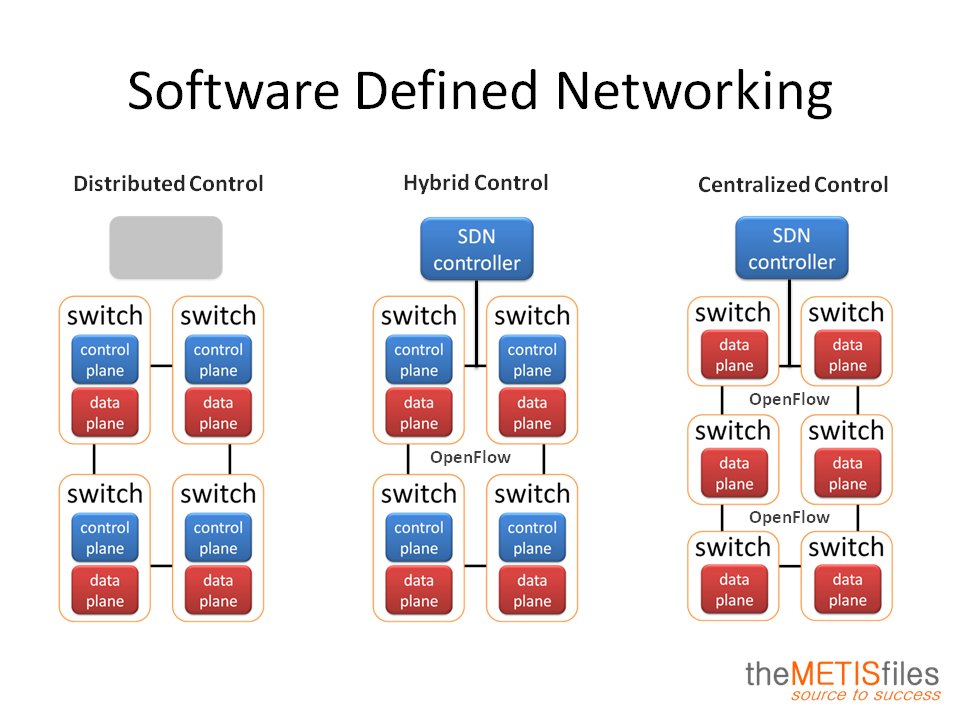
\includegraphics[scale=0.5]{./Drawings/ETSN10-Network_Architecture_Performance/software-defined-networking.png}
  \caption{Software Defined Networking \\ \href{https://www.themetisfiles.com/2012/10/the-future-of-the-network-is-software-defined/}{Source}}
  \label{fig:SDN}
\end{figure}

\paragraph{Network Function Virtualization}\label{par:NFV}
Network Function Virtualization is a massive part in why 5G is going to be able to scale to handle the traffic that will be placed on it.

\begin{definition}[Network Function Virtualization]\label{def:Network_Function_Virtualization}
  \emph{Network Function Virtualization} (\emph{NFV}) is the process of taking functions that used to be performed by dedicated physical entities and virtualizing them.
  This way, there are virtual machines or containers running the same functions as the physical hardware, but multiple instances can run on the same hardware.
  This also allows for dynamic scaling as the network demands.

  \begin{remark}[\nameref*{def:Software_Defined_Networking} Requirement]\label{rmk:NFV_Rely_SDN}
    \nameref{def:Network_Function_Virtualization} can only work because of \nameref{def:Software_Defined_Networking}.
    The only way to be able to move network functions around easily to have the funcctions be software-defined, allowing networks to reconfigure dynamically.
  \end{remark}

  \begin{remark}[Core 5G Functionality]\label{rmk:NFV_Core_5G}
    \nameref{def:Network_Function_Virtualization} is one of the 3 \textbf{MAJOR} functionalities that is enabling 5G to happen.
  \end{remark}
\end{definition}

\paragraph{Network Slicing}\label{par:Network_Slicing}
\begin{definition}[Network Slicing]\label{def:Network_Slicing}
  \emph{Network Slicing} is a network architecture that enables the multiplexing of virtualized and independent logical networks on the same physical network infrastructure.
  Each network slice is an isolated end-to-end network, thus it has its own Quality of Service requirements and management techniques.
  These slices can be tailored to fulfill diverse requirements as requested by a particular application.
  \begin{itemize}[noitemsep]
  \item A mobile broadband slice can handle Quality of Service for video streams.
  \item A URLLC slice can prioritize alarm packets.
  \end{itemize}

  \begin{remark}[Core 5G Functionality]\label{rmk:Network_Slicing_Core_5G}
    \nameref{def:Network_Slicing} is one of the 3 \textbf{MAJOR} functionalities that is enabling 5G to happen.
  \end{remark}
\end{definition}

With \nameref{def:Network_Slicing}, we can have one \nameref{def:Control_Plane} that handles several user slices, or there can be slices that have different dedicated \nameref{def:Control_Plane}s and \nameref{def:Data_Plane}s.

\paragraph{Cloud RAN}\label{par:Cloud_RAN}
\begin{definition}[Cloud Radio Access Network]\label{def:Cloud_RAN}
  In \emph{Cloud Radio Access Network}s (\emph{Cloud RAN}s), the raw radio signal is picked up by the base station and transmitted to a data center backend.
\end{definition}

The advantages of this are:
\begin{itemize}[noitemsep]
\item Performance Gains from cooperation and coordination
\item Shared Resources
\end{itemize}

However, the disadvantages of this are:
\begin{itemize}[noitemsep]
\item There is a single point of failure
\item Needs \textbf{A LOT} of capacity ($\approx 12$ Tbps)
\item Highly vulnerable to problems in the communication network from the base station to the data center.
\end{itemize}

\paragraph{Frame Structure}\label{par:Frame_Structure}
In 5G, each frame is \SI{10}{\milli{} \second{}}, and each subframe is \SI{1}{\milli{} \second{}}, like in \nameref{def:LTE}.

However, the structure of the frame is \textbf{much more} flexible, with the subcarrier spacing, slots per subframe, and slot lengths being dynamic.
The combination of these parameters is called numerology.

\begin{table}[h!tbp]
  \centering
  \begin{tabular}{cccc}
    \toprule
    \textbf{Numerology} & \textbf{Subcarrier Spacing} & \textbf{Slots Per Subframe} & \textbf{Slot Length} \\
    \midrule
    0 & \SI{15}{\kilo{} \hertz{}} & 1 & \SI{1}{\milli{} \second{}} \\
    1 & \SI{30}{\kilo{} \hertz{}} & 2 & \SI{500}{\micro{} \second{}} \\
    2 & \SI{60}{\kilo{} \hertz{}} & 4 & \SI{250}{\micro{} \second{}} \\
    3 & \SI{120}{\kilo{} \hertz{}} & 8 & \SI{125}{\micro{} \second{}} \\
    \bottomrule
  \end{tabular}
  \caption{5G Numerology}
  \label{tab:5G_Numerology}
\end{table}

\begin{remark*}
  Different numerologies cannot be used by the same network slice, but different numerologies can be used by \textbf{different} network slices in the same frame.
\end{remark*}

The advantage of these different numerologies can be shown best by examples:
\begin{itemize}[noitemsep]
\item A URLLC application such as industrial control might need a short slot time to ensure low latency.
\item An eMBB application such as UHD video streaming might want a large slot capacity (low overhead for large amounts of data transmitted).
\item An mMTC application such as an IoT sensor network might need many small slots to allocate small amounts of data to each device.
\end{itemize}

\paragraph{Slot Format}\label{par:Slot_Format}
In 5G, the format inside of the individual slots is also more flexible.
\textbf{Each symbol} in a given slot can be allocated to:
\begin{itemize}[noitemsep]
\item The uplink
\item The Downlink
\item Both (Allocated dynamically as needed)
\end{itemize}

This is a stark contrast to \nameref{def:LTE}, which requires that every symbol in a slot be the same.

In total 5G defines 61 different slot formats, combinations of uplink, downlink, and flexible symbols.

\paragraph{Resource Allocation in 5G}\label{par:5G_Resource_Allocation}
In 5G NR, resources are allocated in resource blocks ($RB$), similarly to \nameref{def:LTE}.
The difference is that the number and size of resource blocks in a slot varies.

With a normal cyclic prefix length, the minimum number of $RB$s in a slot is 24, and the maximum is 275.
Each RB consists of 12 subcarriers and 14 symbols, but the subcarrier spacing and symbol duration depends on the numerology.

So some resource blocks are in effect more “valuable” than others, in terms of their scarcity (how many are in the slot), and capacity (the amount of data that can be sent in one RB).

\paragraph{Enabling Technologies for 5G}\label{par:5G_Enabling_Technologies}
To make 5G work, there are some technologies in use that are enabling the higher data speeds and greater functionality required.
Each of these is important, and it is likely that all 3 will be used together to ensure the system works well.
\begin{enumerate}[noitemsep]
\item \nameref{subpar:Millimeter_Wave}
\item \nameref{subpar:Small_Cells}
\item \nameref{subpar:Massive_MIMO}
\end{enumerate}

\subparagraph{Millimeter Wave}\label{subpar:Millimeter_Wave}
\textbf{TODO!!}

\subparagraph{Small Cells}\label{subpar:Small_Cells}
\textbf{TODO!!}

\subparagraph{Massive MIMO}\label{subpar:Massive_MIMO}
\textbf{TODO!!}

%%% Local Variables:
%%% mode: latex
%%% TeX-master: "../../ETSN10-Network_Architecture_Performance-Reference_Sheet"
%%% End:
